\documentclass[12pt, fleqn]{article}

\usepackage[utf8]{inputenc}
\usepackage{graphicx}
\usepackage{paralist}
\usepackage{booktabs}
\usepackage{hyperref}
\usepackage{amsmath}
\usepackage{amsfonts}
\usepackage{amssymb}
\usepackage{amsthm}
\usepackage{color}
\usepackage[nounderscore]{syntax}
\usepackage{mdwtab}
\usepackage{mathpartir}
\usepackage[pdf]{graphviz}

% \renewcommand{\texttt}[1]{\OldTexttt{\color{teal}{#1}}}
\newcommand{\pnote}[1]{{\langle \text{#1} \rangle}}
\newcommand{\mname}[1]{\mbox{\sf #1}}
\definecolor{mGreen}{rgb}{0,0.6,0}
\definecolor{mGray}{rgb}{0.5,0.5,0.5}
\definecolor{mPurple}{rgb}{0.58,0,0.05}
\definecolor{mGreen2}{rgb}{0.05,0.65,0.05}
\definecolor{mGray2}{rgb}{0.55,0.55,0.55}
\definecolor{mPurple2}{rgb}{0.63,0.05,0.05}
\definecolor{backgroundColour}{rgb}{0.95,0.95,0.92}
\definecolor{backgroundColour2}{rgb}{0.95,0.92,0.95}

\definecolor{t_comment}{rgb}{0.2,1,0.2}
\definecolor{t_mGray}{rgb}{0.5,0.5,0.5}
\definecolor{t_mPurple}{rgb}{0.58,0,0.05}
\definecolor{t_blue}{rgb}{0.4,0.6,0.8}
\definecolor{t_mGreen2}{rgb}{0.05,0.65,0.05}
\definecolor{t_mGray2}{rgb}{0.75,0.75,0.75}
\definecolor{t_mPurple2}{rgb}{0.63,0.05,0.05}
\definecolor{t_bg}{rgb}{0.15,0.15,0.18}

\setlength{\parindent}{0pt}
\setlength {\topmargin} {-.15in}
\oddsidemargin 0mm
\evensidemargin 0mm
\textwidth 160mm
\textheight 200mm

\pagestyle {plain}
\pagenumbering{arabic}

\newcounter{stepnum}

\title{2MI3 Assignment 4 Solution}
\author{x}
\date{\today}

\begin{document}


\begin{center}

    {\large \textbf{COMPSCI 3MI3}}\\[8mm]
    {\huge \textbf{Assignment 4}}\\[6mm]
  
\end{center}

\section{Solution Set}

\subsection{Q1}

\begin{enumerate}[(a)]
    \item
    \begin{center}
        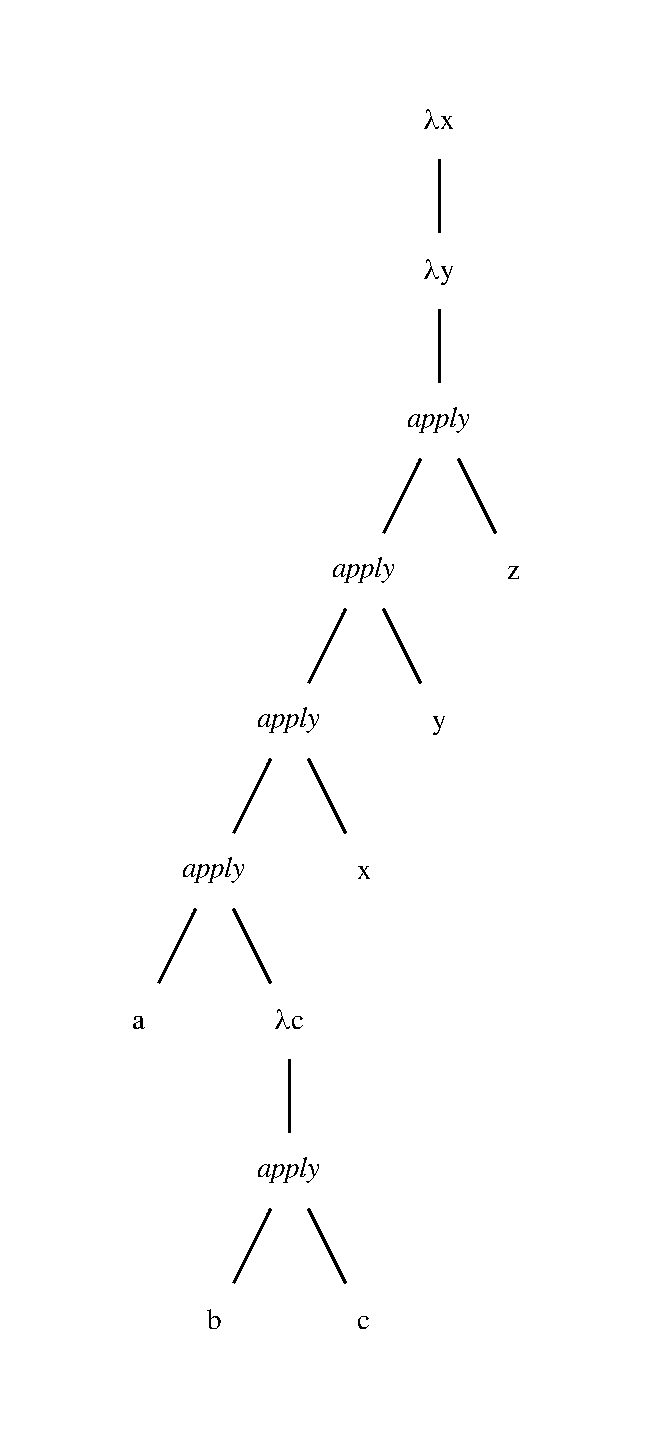
\includegraphics[width=0.43\textwidth]{a1.pdf}
    \end{center}

    \item
    \begin{center}
        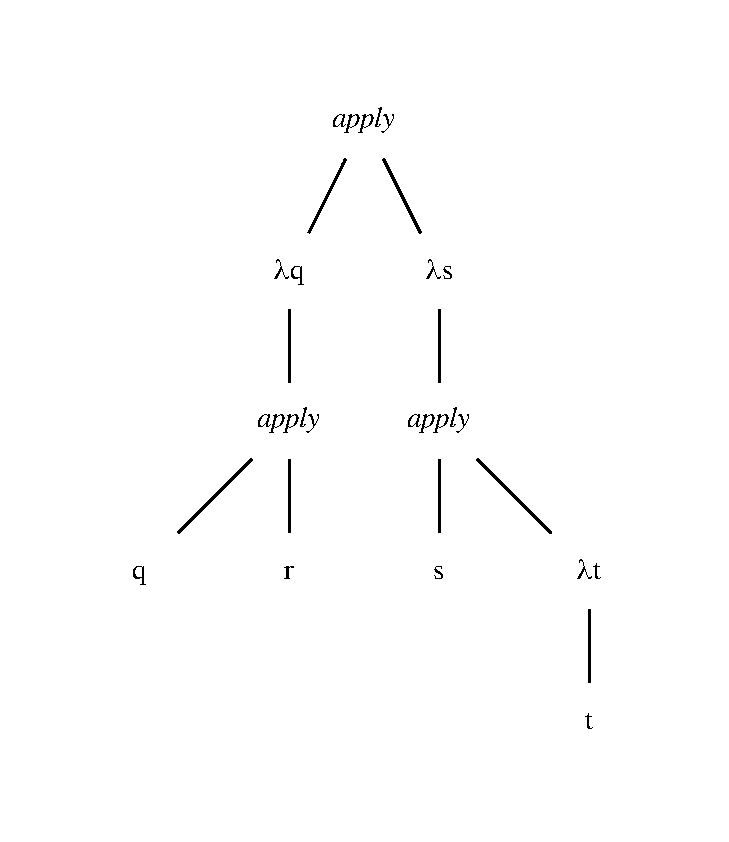
\includegraphics[width=0.53\textwidth]{b1.pdf}
    \end{center}
    
    \item
    \begin{center}
        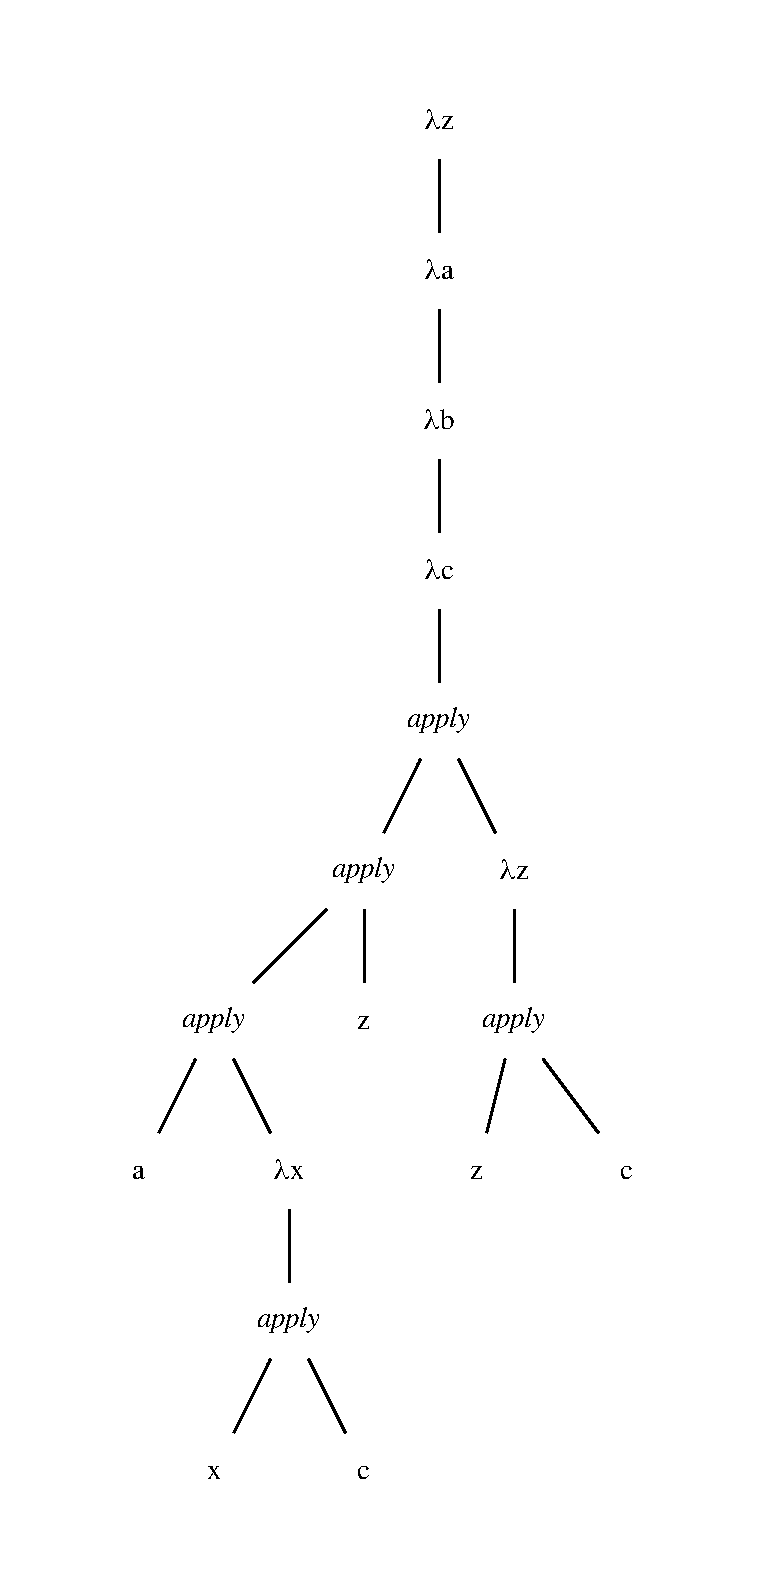
\includegraphics[width=0.52\textwidth]{c1.pdf}
    \end{center} 

\end{enumerate}

\subsection{Q2}
We define a lambda expression which performs logical or over Church Booleans as follows:
\begin{center}
    $\texttt{or} = \lambda b. \lambda c.\:b\:\texttt{tru}\:c$
\end{center}
We can prove our operation works for all possible inputs.

\medskip

\underline{With input \texttt{tru} \texttt{tru}:}
\begin{center}
    \begin{tabular}{c l}
    & $(\lambda b. \lambda c.\:b\:\texttt{tru}\:c)\:\texttt{tru}\:\texttt{tru}$ \\ 
    $\rightarrow$ & $(\lambda c.\:\texttt{tru}\:\texttt{tru}\:c)\:\texttt{tru}$ \\
    $\rightarrow$ & $\texttt{tru}\:\texttt{tru}\:\texttt{tru}$ \\
    $\rightarrow$ & $(\lambda t. \lambda f. t)\:\texttt{tru}\:\texttt{tru}$ \\
    $\rightarrow$ & $(\lambda f. \texttt{tru})\:\texttt{tru}$ \\
    $\rightarrow$ & $\texttt{tru}$ \\
    $\nrightarrow$ & \\
    \end{tabular}
\end{center}
    
\underline{With input \texttt{tru} \texttt{fls}:}
\begin{center}
    \begin{tabular}{c l}
    & $(\lambda b. \lambda c.\:b\:\texttt{tru}\:c)\:\texttt{tru}\:\texttt{fls}$ \\ 
    $\rightarrow$ & $(\lambda c.\:\texttt{tru}\:\texttt{tru}\:c)\:\texttt{fls}$ \\
    $\rightarrow$ & $\texttt{tru}\:\texttt{tru}\:\texttt{fls}$ \\
    $\rightarrow$ & $(\lambda t. \lambda f. t)\:\texttt{tru}\:\texttt{fls}$ \\
    $\rightarrow$ & $(\lambda f. \texttt{tru})\:\texttt{fls}$ \\
    $\rightarrow$ & $\texttt{tru}$ \\
    $\nrightarrow$ & \\
    \end{tabular}
\end{center}

\underline{With input \texttt{fls} \texttt{tru}:}
\begin{center}
    \begin{tabular}{c l}
    & $(\lambda b. \lambda c.\:b\:\texttt{tru}\:c)\:\texttt{fls}\:\texttt{tru}$ \\ 
    $\rightarrow$ & $(\lambda c.\:\texttt{fls}\:\texttt{tru}\:c)\:\texttt{tru}$ \\
    $\rightarrow$ & $\texttt{fls}\:\texttt{tru}\:\texttt{tru}$ \\
    $\rightarrow$ & $(\lambda t. \lambda f. f)\:\texttt{tru}\:\texttt{tru}$ \\
    $\rightarrow$ & $(\lambda f. f)\:\texttt{tru}$ \\
    $\rightarrow$ & $\texttt{tru}$ \\
    $\nrightarrow$ & \\
    \end{tabular}
\end{center}

\underline{With input \texttt{fls} \texttt{fls}:}
\begin{center}
    \begin{tabular}{c l}
    & $(\lambda b. \lambda c.\:b\:\texttt{tru}\:c)\:\texttt{fls}\:\texttt{fls}$ \\ 
    $\rightarrow$ & $(\lambda c.\:\texttt{fls}\:\texttt{tru}\:c)\:\texttt{fls}$ \\
    $\rightarrow$ & $\texttt{fls}\:\texttt{tru}\:\texttt{fls}$ \\
    $\rightarrow$ & $(\lambda t. \lambda f. f)\:\texttt{tru}\:\texttt{fls}$ \\
    $\rightarrow$ & $(\lambda f. f)\:\texttt{fls}$ \\
    $\rightarrow$ & $\texttt{fls}$ \\
    $\nrightarrow$ & \\
    \end{tabular}
\end{center}


\subsection{Q3}

We define a lambda expression which performs exponentiation over Church Numerals, such that
\texttt{$m^n$} is represented \verb|exp m n| where \verb|exp| is defined as
\begin{center}
    $\texttt{exp} = \lambda m. \lambda n.\:n\:m$
\end{center}

\medskip
We will prove our operation works with inputs $c_2$, $c_2$ to evaluate $2^2$.

\medskip

\underline{With input \texttt{$c_2$} \texttt{$c_2$}:}
\begin{center}
    \begin{tabular}{c l}
    & $(\lambda m. \lambda n.\:n\:m)\:c_2\:c_2$ \\ 
    $\rightarrow$ $\rightarrow$ & $(\lambda s. \lambda z.\:s\:(s\:z)) (\lambda a.\lambda b.\:a\:(a\:b))$ \\
    $\rightarrow$ & $\lambda z.\: (\lambda a.\lambda b.\:a\:(a\:b))\:((\lambda a.\lambda b.\:a\:(a\:b))\:z)$ \\
    $\rightarrow$ & $\lambda z.\: (\lambda a.\lambda b.\:a\:(a\:b))\:(\lambda c.\:z\:(z\:c))$ \\
    $\rightarrow$ & $\lambda z.\lambda b.\:(\lambda c.\:z\:(z\:c))\:((\lambda c.\:z\:(z\:c))\:b)$ \\
    $\rightarrow$ & $\lambda z.\lambda b.\:(\lambda c.\:z\:(z\:c))\:(z\:(z\:b))$ \\
    $\rightarrow$ & $\lambda z.\lambda b.\:z\:(z\:(z\:(z\:b)))$ \\
    $\nrightarrow$ & \\
    \end{tabular}
\end{center}

Our result is equivalent to $\lambda s.\: \lambda z.\:s\:(s\:(s\:(s\:z)))$ which is $c_4$. Thus we can conclude our exponential expression
works for inputs $c_2$, $c_2$.

\end {document}